% Chapter Template

\chapter{Flip-flop qubit measurements} % Main chapter title

\label{Chapter7} % Change X to a consecutive number; for referencing this chapter elsewhere, use \ref{ChapterX}

\HRule
\vspace{0.5cm} \hspace{2cm}
\small
\hangindent=4cm
\\
        ``\emph{hopefully sth here...}"
\\ \\
\hangindent=4cm
\begin{flushright}
--? \\
\end{flushright}

\vspace{0.5cm}

\noindent \HRule
\clearpage

\section{Proof of principle Flip-flop measurement} \label{sec:ff_resonance}

\begin{figure}
	\centering
	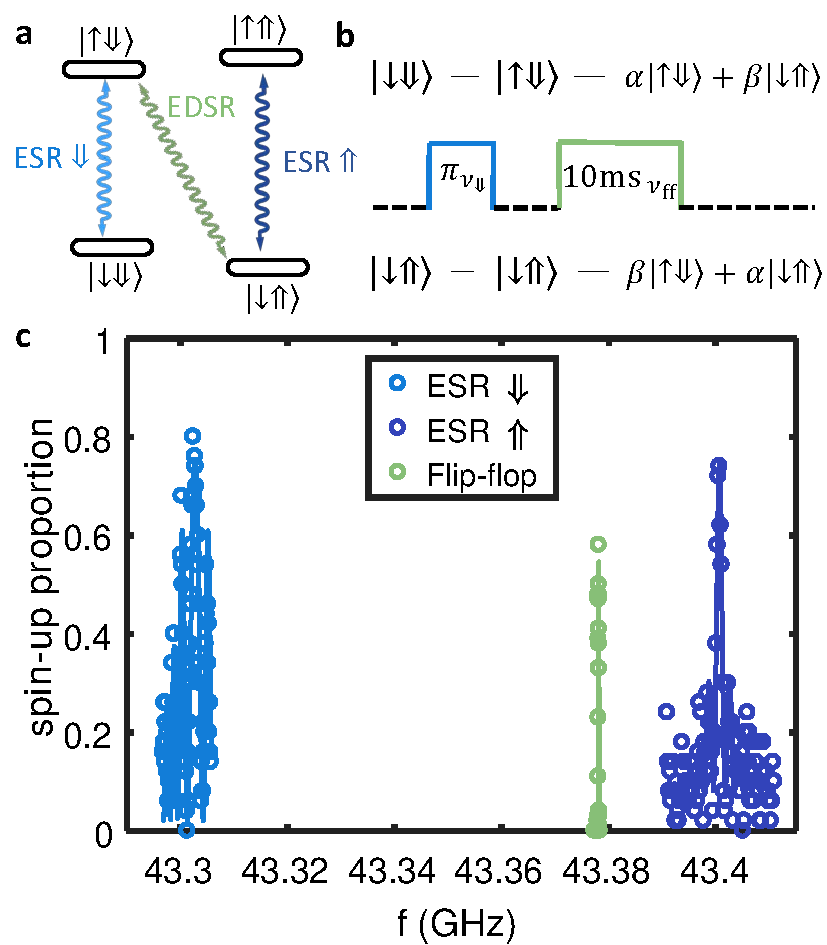
\includegraphics[width=0.9\textwidth]{polished/FF_spectrum.pdf}
	\caption[Flip-flop qubit resonance]{\textbf{Flip-flop qubit resonance. a}}
	\label{fig:ff_spectrum}
\end{figure}

\section{Dipole-dipole coupling devices} \label{sec:dd_meas}

\begin{figure}
	\centering
	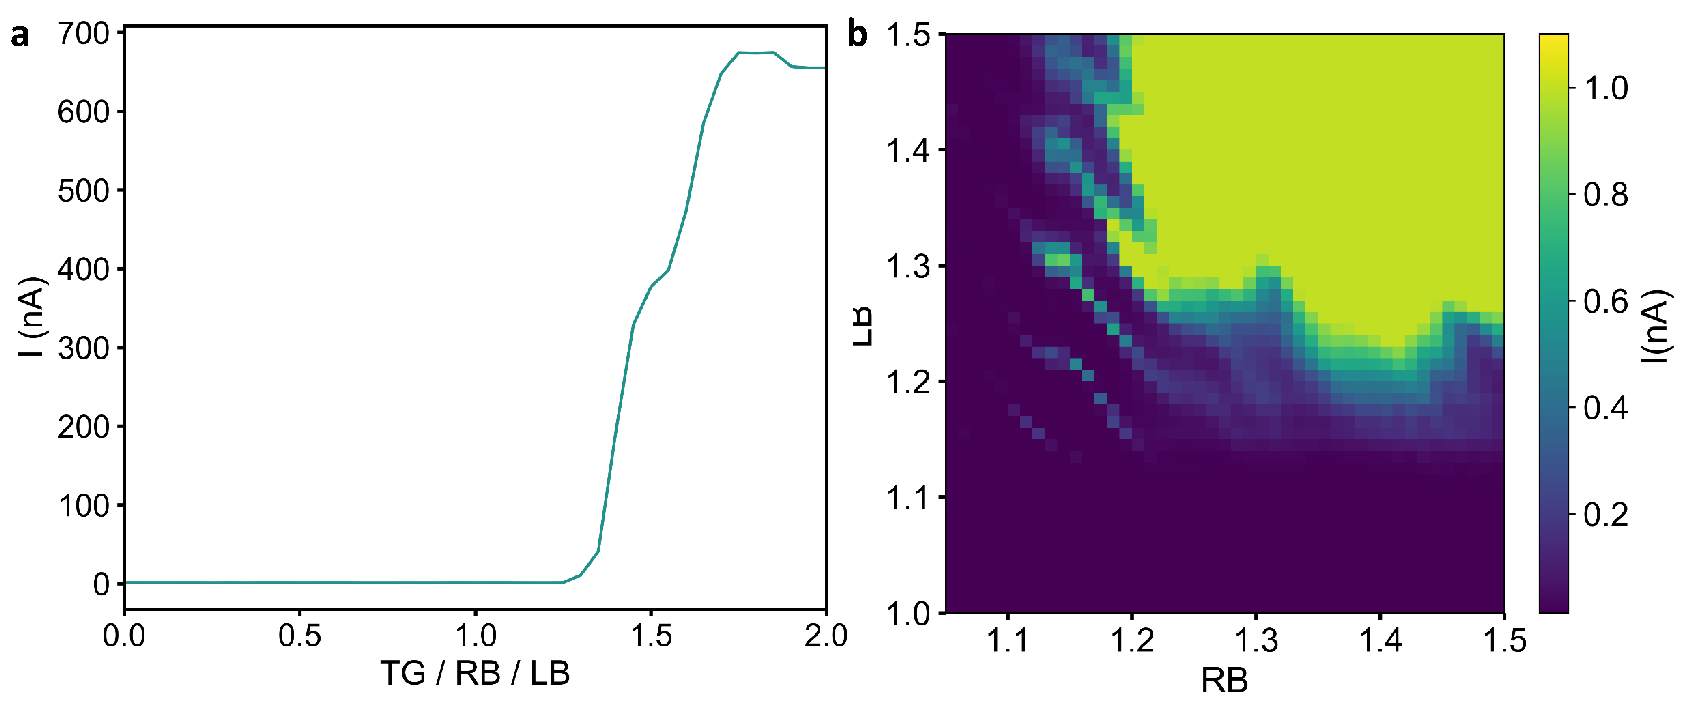
\includegraphics[width=\textwidth]{polished/turnon_pinchoff.pdf}
	\caption[Flip-flop qubit turn on and pinch-off]{\textbf{Flip-flop qubit turn on and pinch-off. a}}
	\label{fig:turnon_pinchoff}
\end{figure}

\begin{figure}
	\centering
	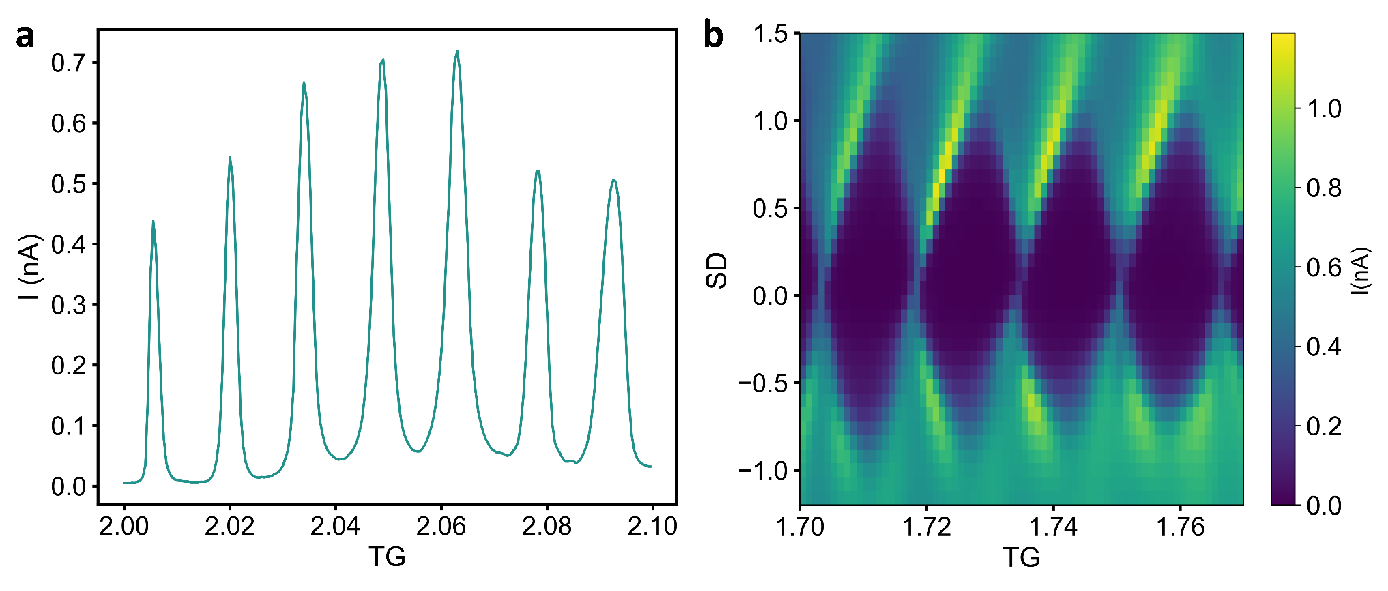
\includegraphics[width=\textwidth]{polished/CoulombOscillations.pdf}
	\caption[Flip-flop qubit Coulomb oscillations and diamonds]{\textbf{Flip-flop qubit Coulomb oscillations and Coulomb diamonds. a}}
	\label{fig:coulomb_oscillations}
\end{figure}

\begin{figure}
	\centering
	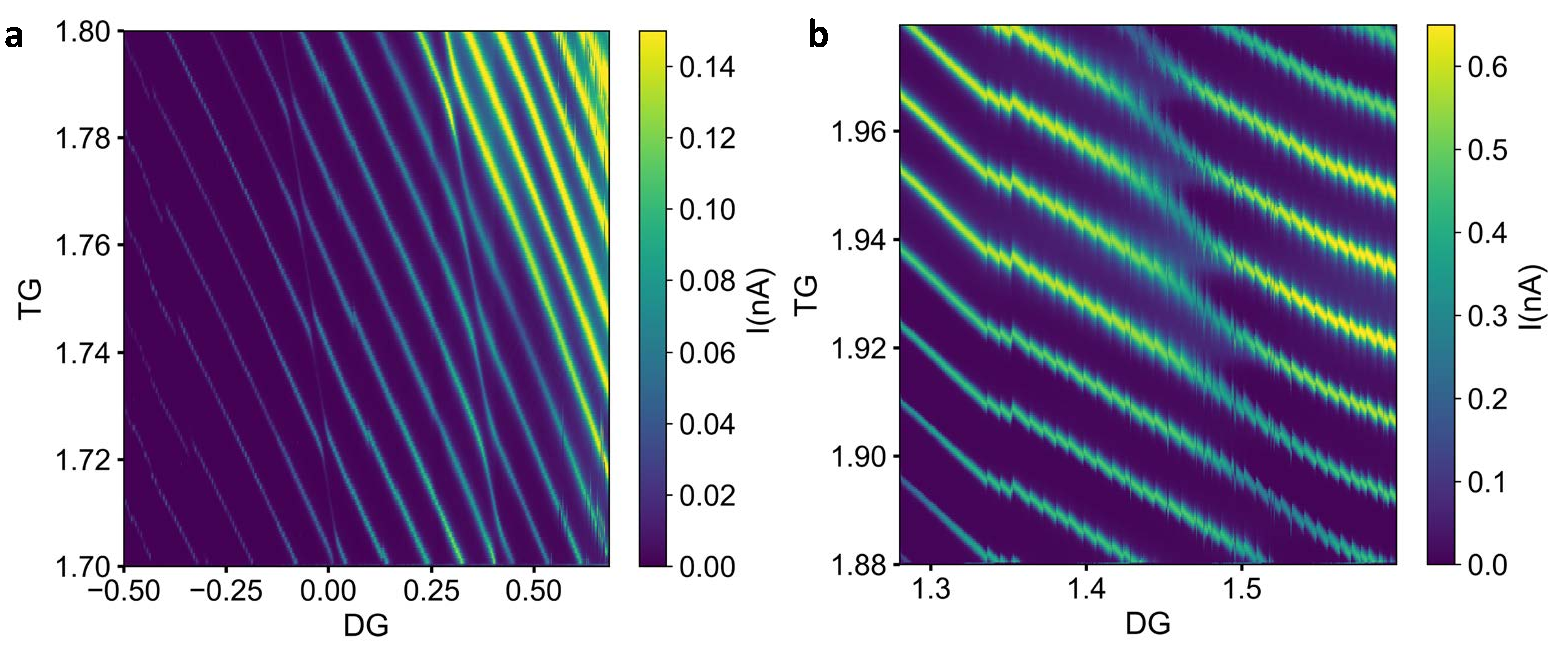
\includegraphics[width=\textwidth]{polished/stability_diagram_ff.pdf}
	\caption[Flip-flop qubit charge stability diagram]{\textbf{Flip-flop qubit charge stability diagram. a}}
	\label{fig:coulomb_oscillations}
\end{figure}


\section{CPWR devices} \label{sec:cpwr_meas}

\subsection{Resonator characterization}

\begin{figure}
	\centering
	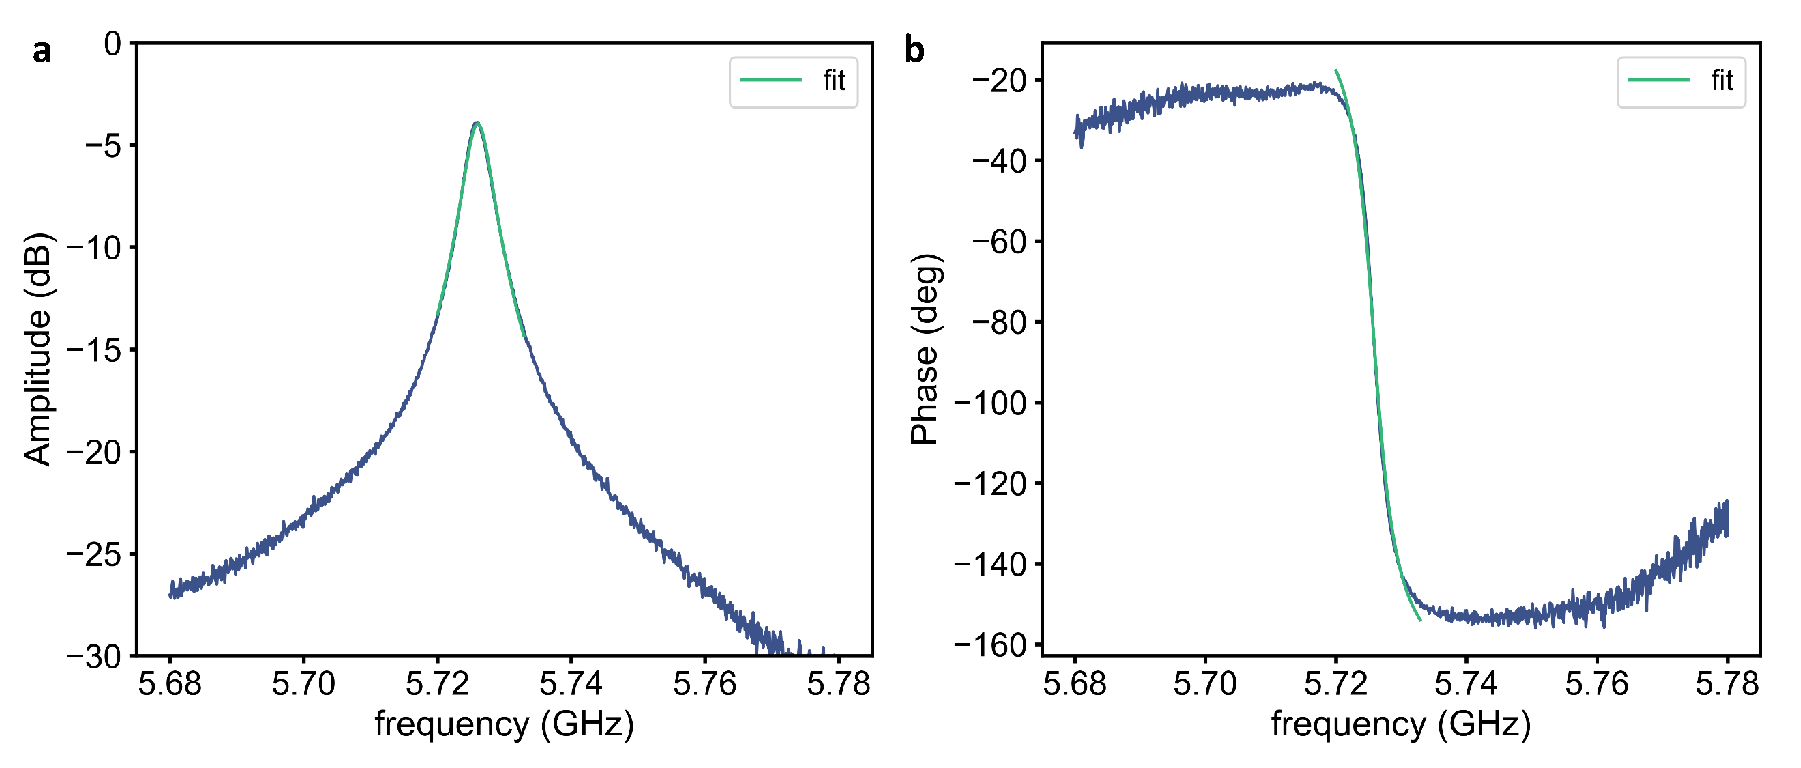
\includegraphics[width=\textwidth]{polished/resonance_fit.pdf}
	\caption[Flip-flop qubit turn on and pinch-off]{\textbf{Flip-flop qubit turn on and pinch-off. a}}
	\label{fig:resonance_fit}
\end{figure}

\begin{figure}
	\centering
	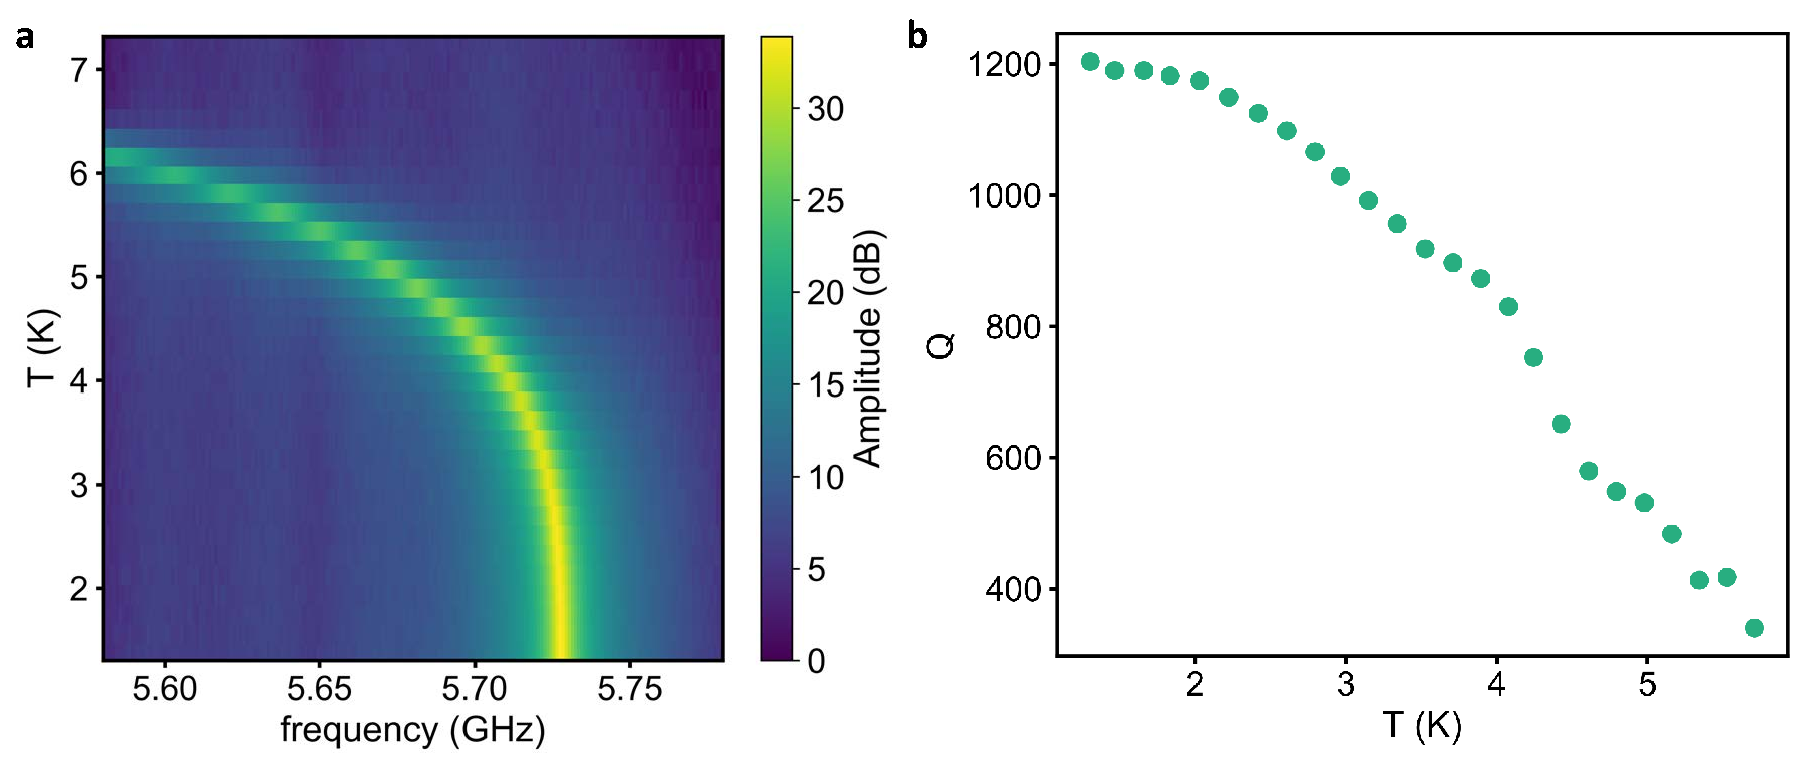
\includegraphics[width=\textwidth]{polished/cpwr_temp.pdf}
	\caption[Flip-flop qubit turn on and pinch-off]{\textbf{Flip-flop qubit turn on and pinch-off. a}}
	\label{fig:cpwr_temp}
\end{figure}

\begin{figure}
	\centering
	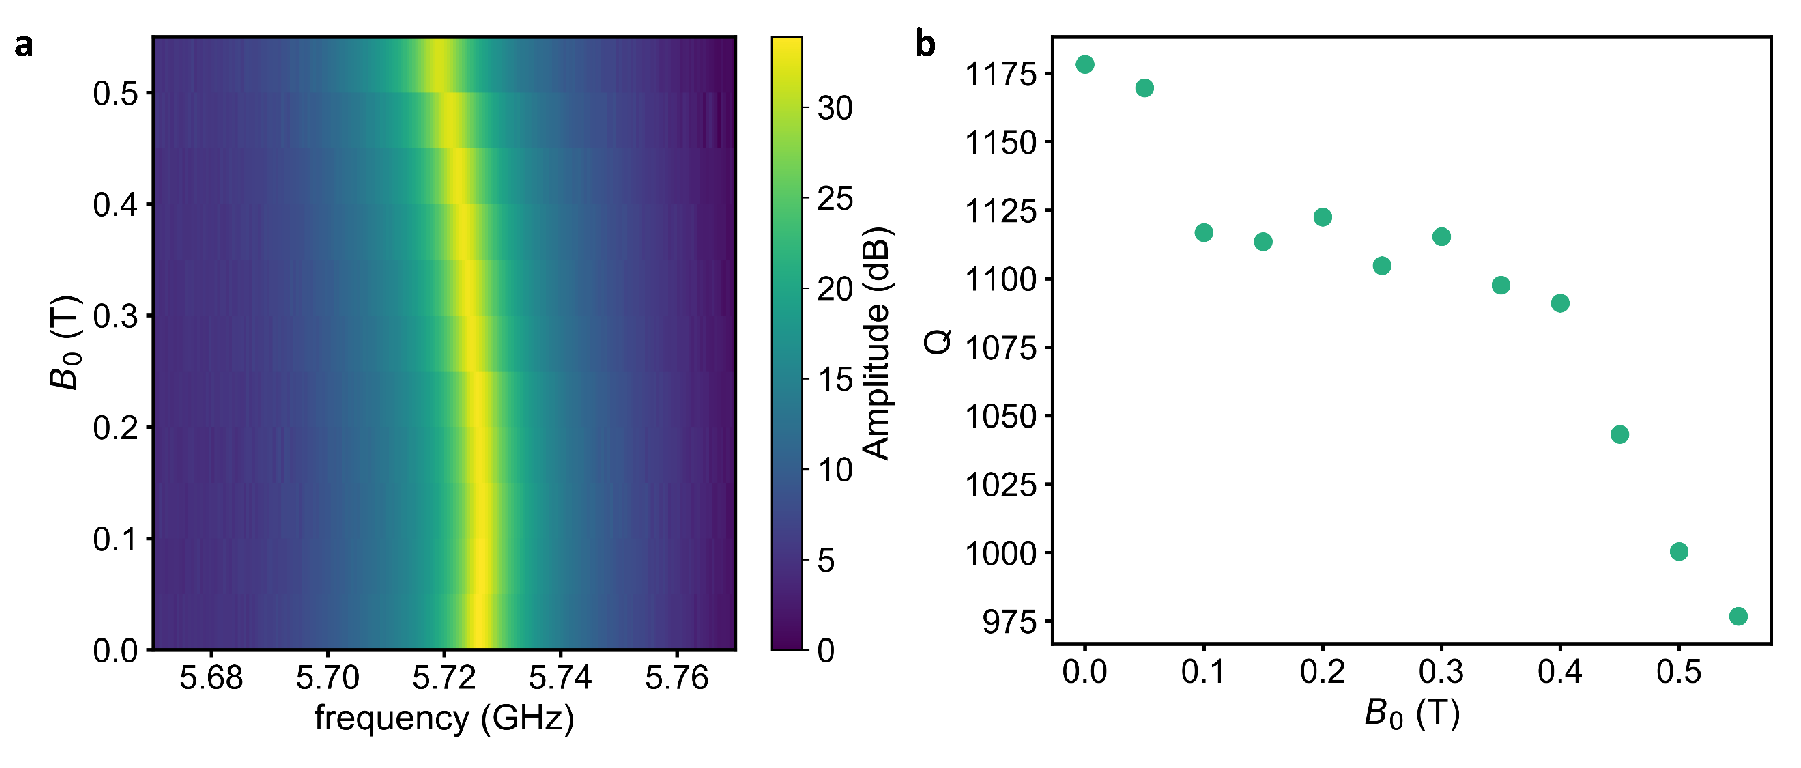
\includegraphics[width=\textwidth]{polished/cpwr_bfield.pdf}
	\caption[Flip-flop qubit turn on and pinch-off]{\textbf{Flip-flop qubit turn on and pinch-off. a}}
	\label{fig:cpwr_bfield}
\end{figure}



\subsection{2DEG influence}

\subsubsection{Low Q}

\begin{figure}
	\centering
	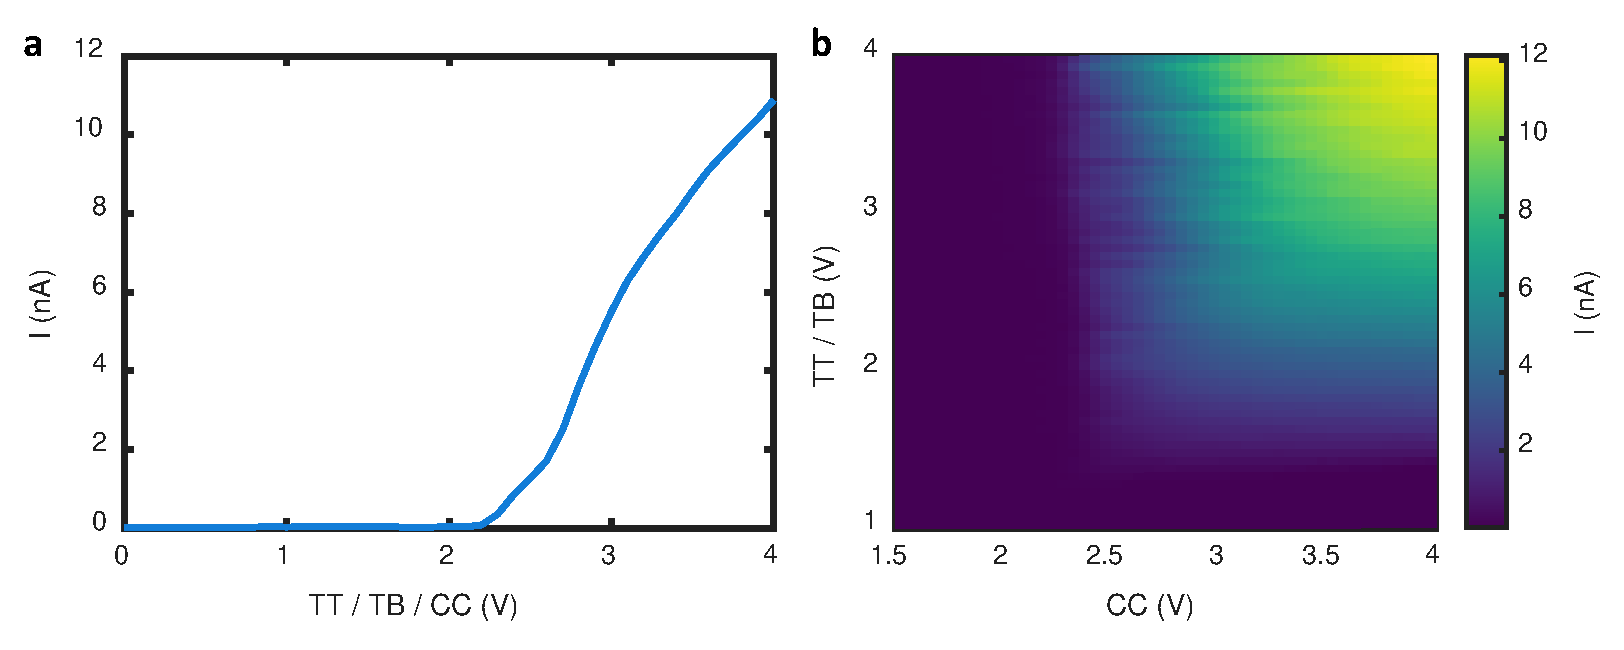
\includegraphics[width=\textwidth]{polished/ResonanceTurnon.pdf}
	\caption[Flip-flop qubit turn on and pinch-off]{\textbf{Flip-flop qubit turn on and pinch-off. a}}
	\label{fig:lowq_turnon}
\end{figure}

\begin{figure}
	\centering
	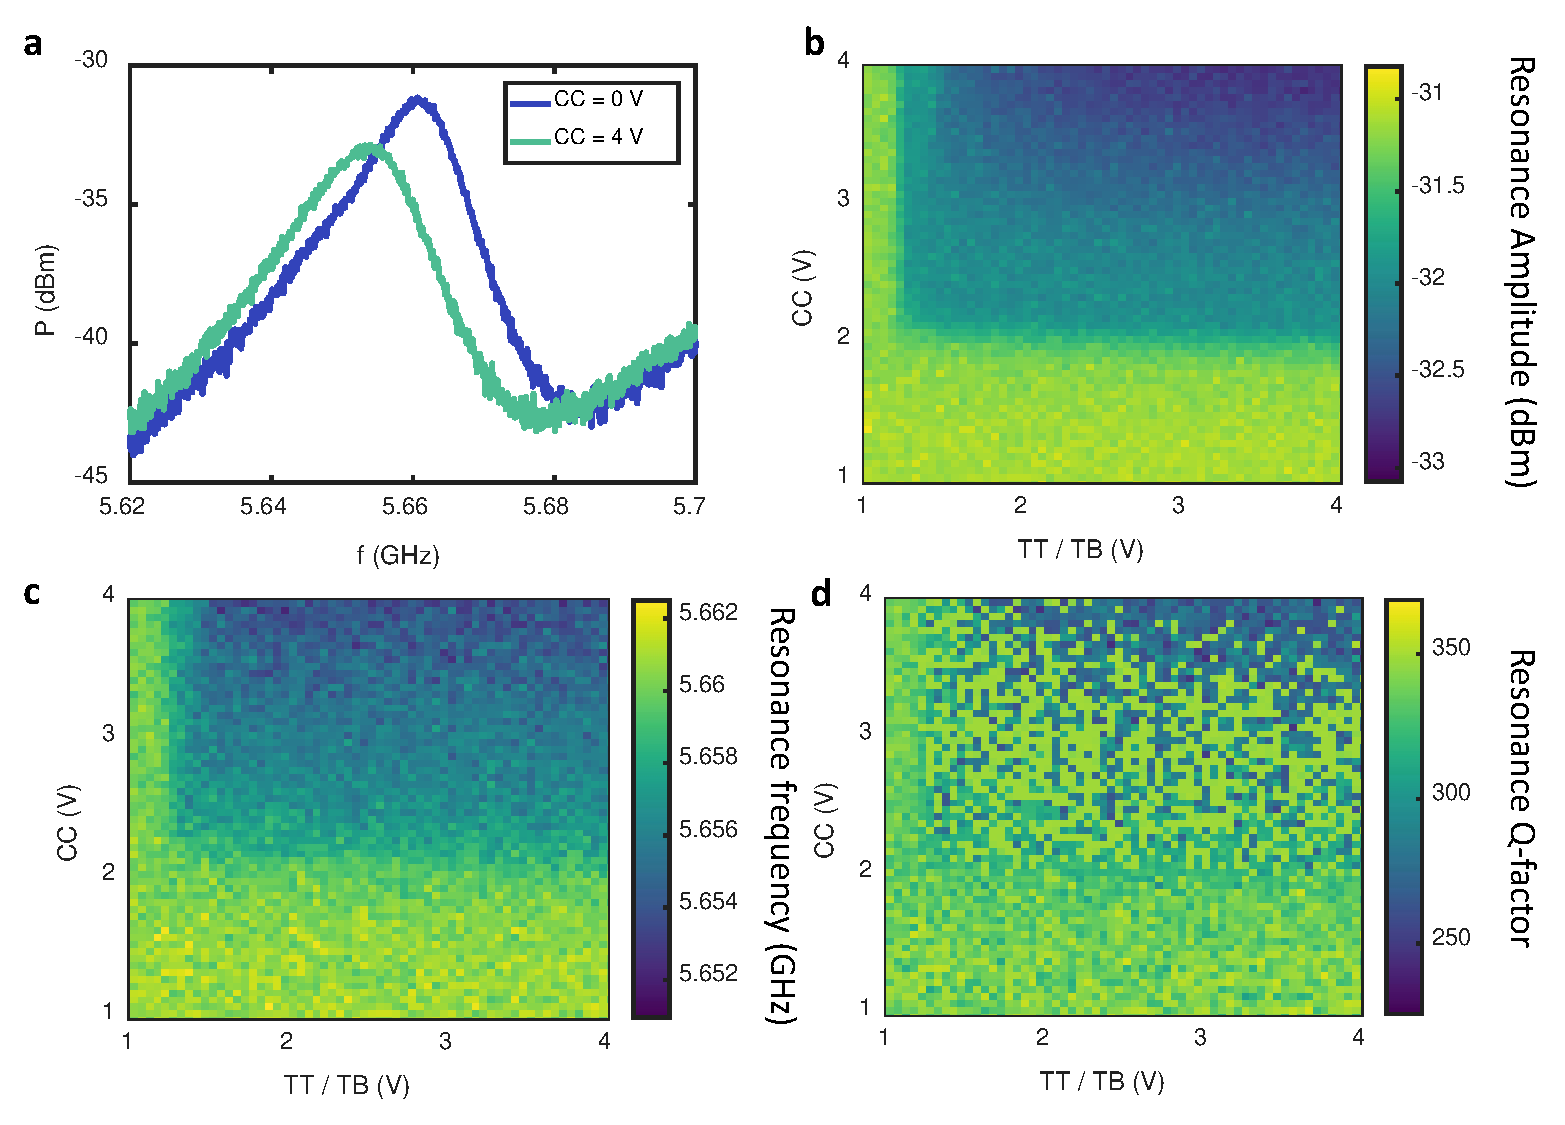
\includegraphics[width=\textwidth]{polished/Resonance2DEG.pdf}
	\caption[Flip-flop qubit turn on and pinch-off]{\textbf{Flip-flop qubit turn on and pinch-off. a}}
	\label{fig:lowq_2deg}
\end{figure}

\subsubsection{High Q}

\begin{figure}
	\centering
	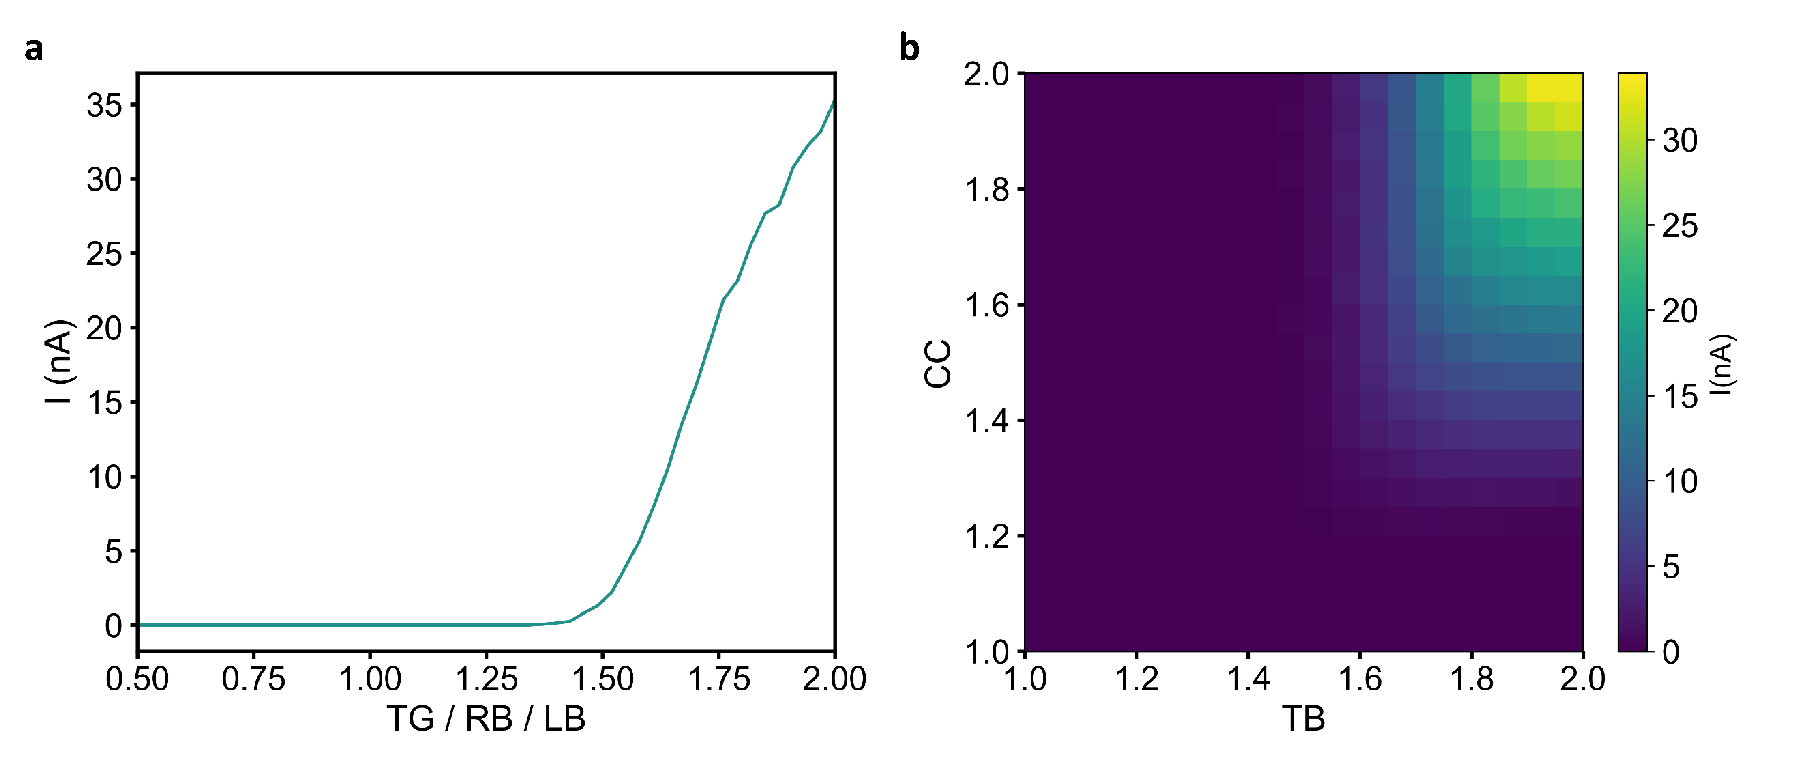
\includegraphics[width=\textwidth]{polished/highq_turnon.pdf}
	\caption[Flip-flop qubit turn on and pinch-off]{\textbf{Flip-flop qubit turn on and pinch-off. a}}
	\label{fig:highq_turnon}
\end{figure}

\begin{figure}
	\centering
	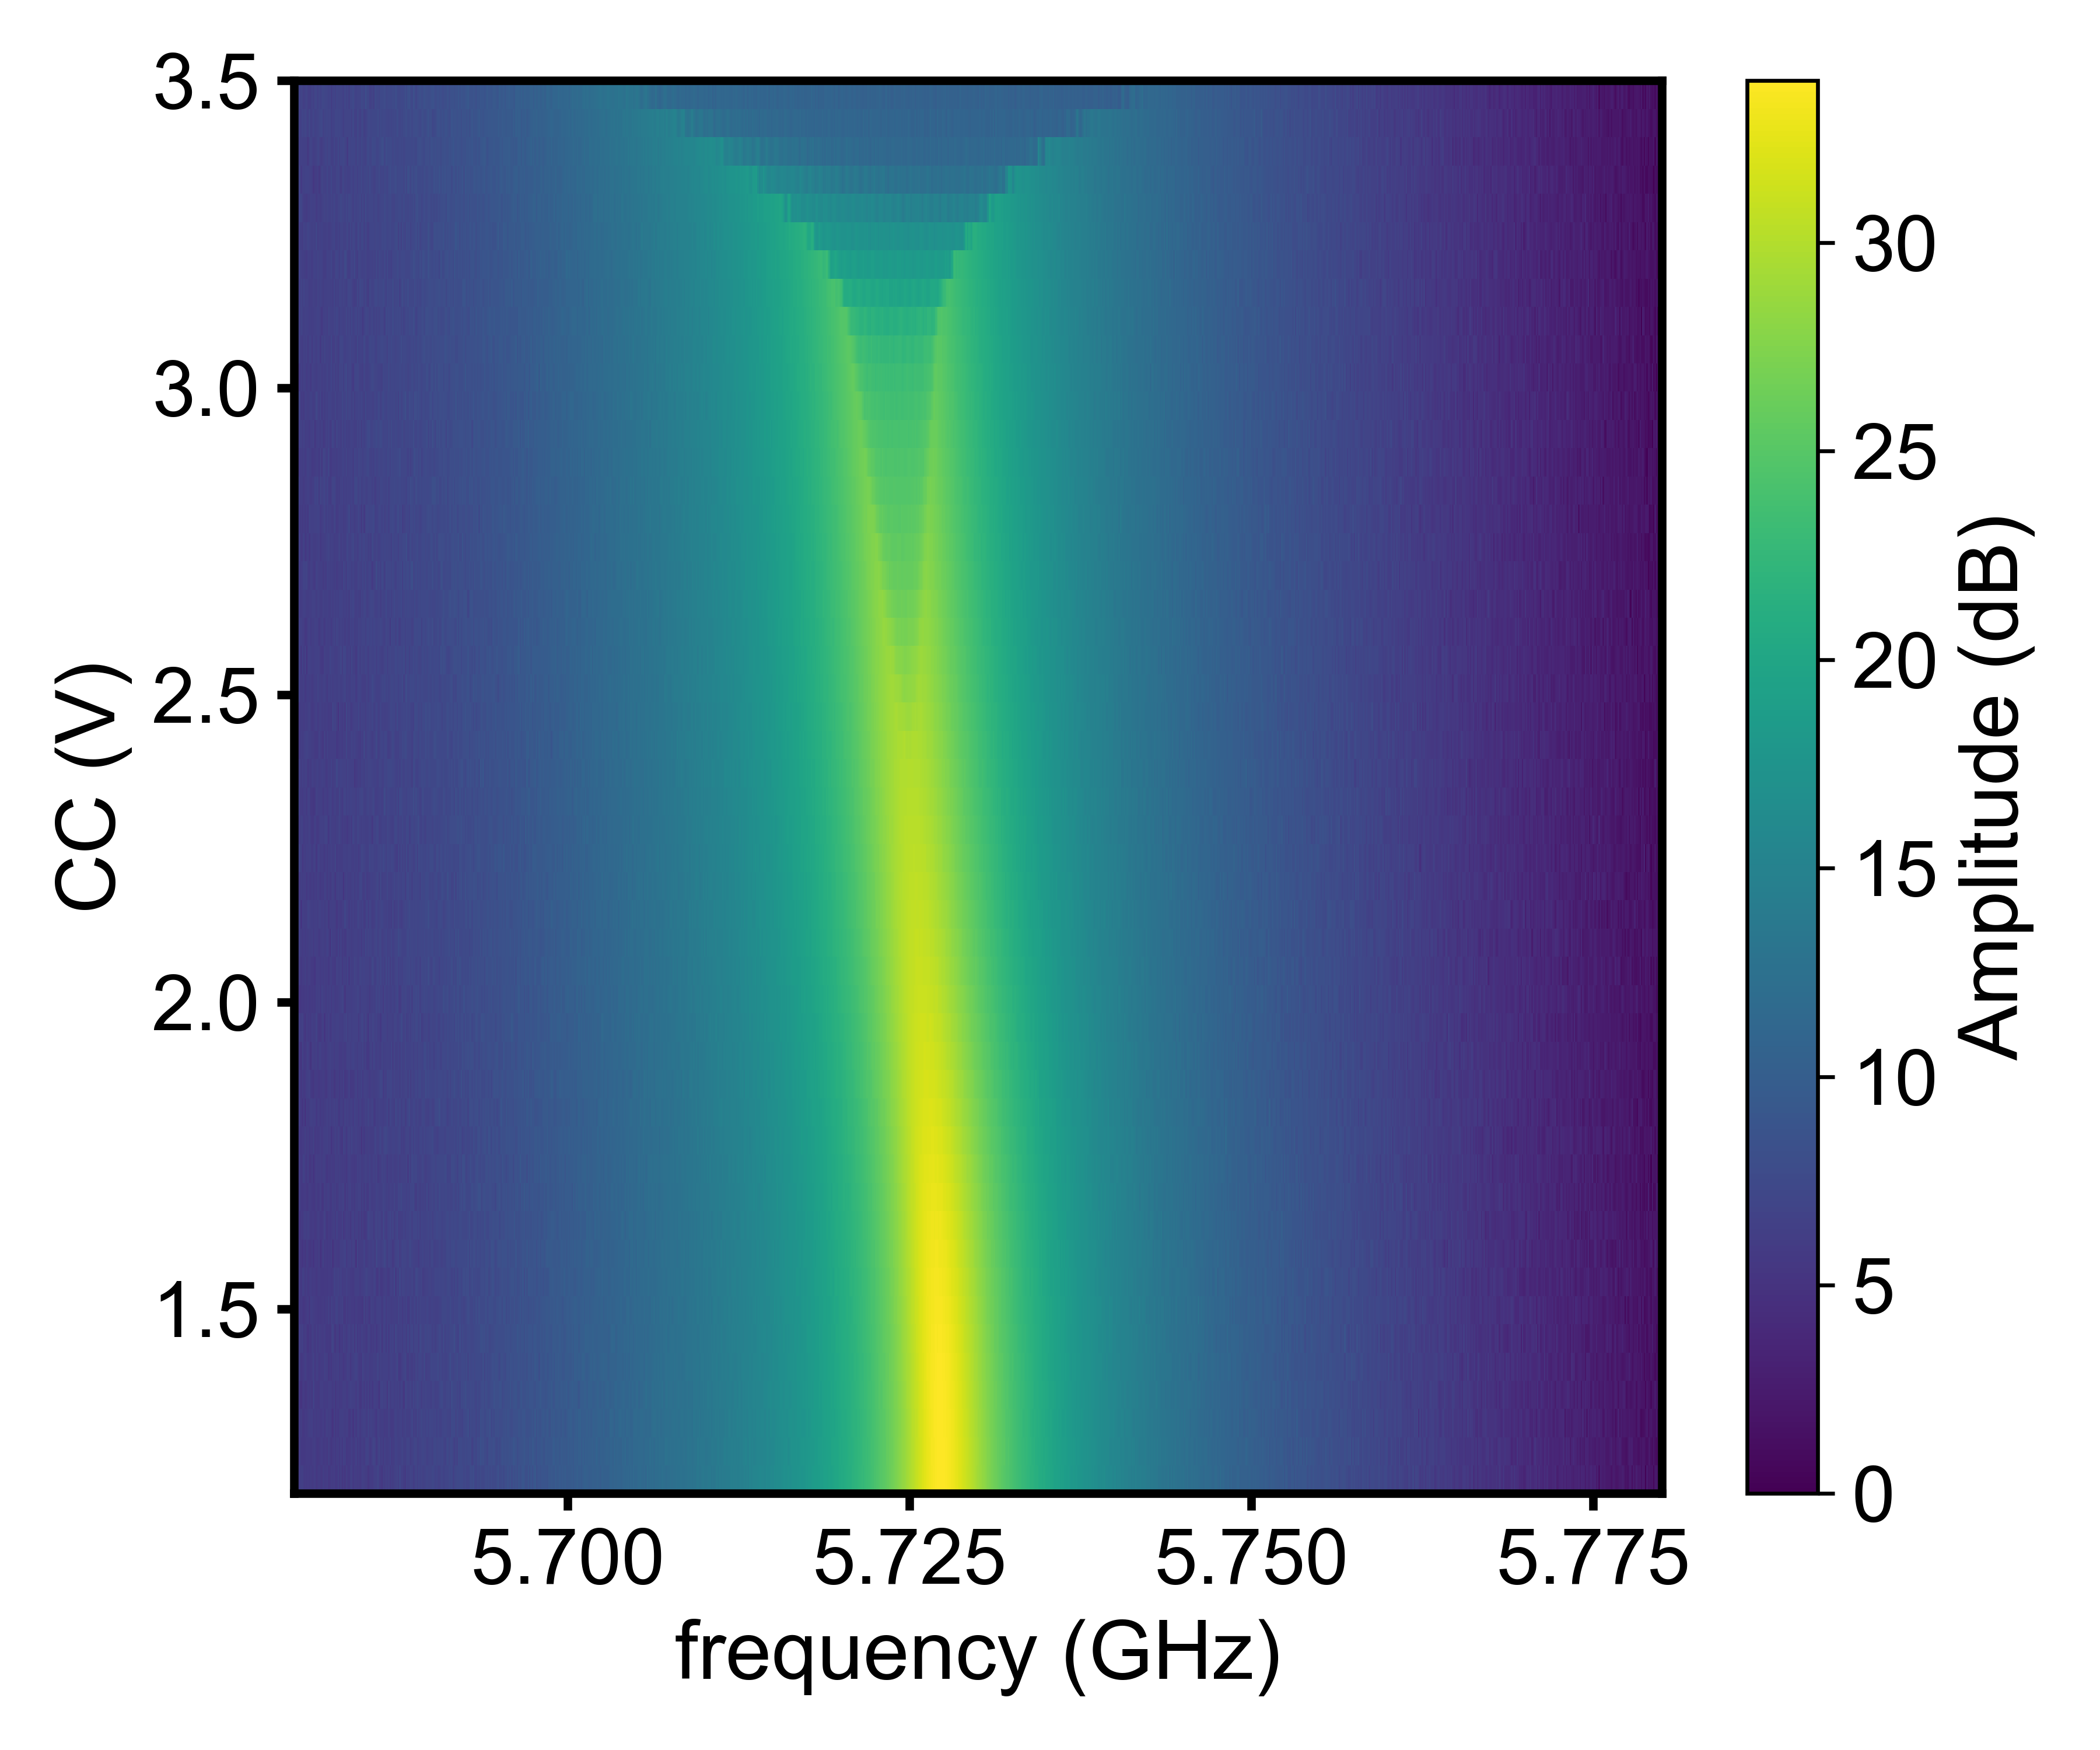
\includegraphics[width=0.6\textwidth]{polished/2deg_mag.png}
	\caption[Flip-flop qubit turn on and pinch-off]{\textbf{Flip-flop qubit turn on and pinch-off. a}}
	\label{fig:highq_2deg}
\end{figure}

\subsection{Power influence}


\begin{figure}
	\centering
	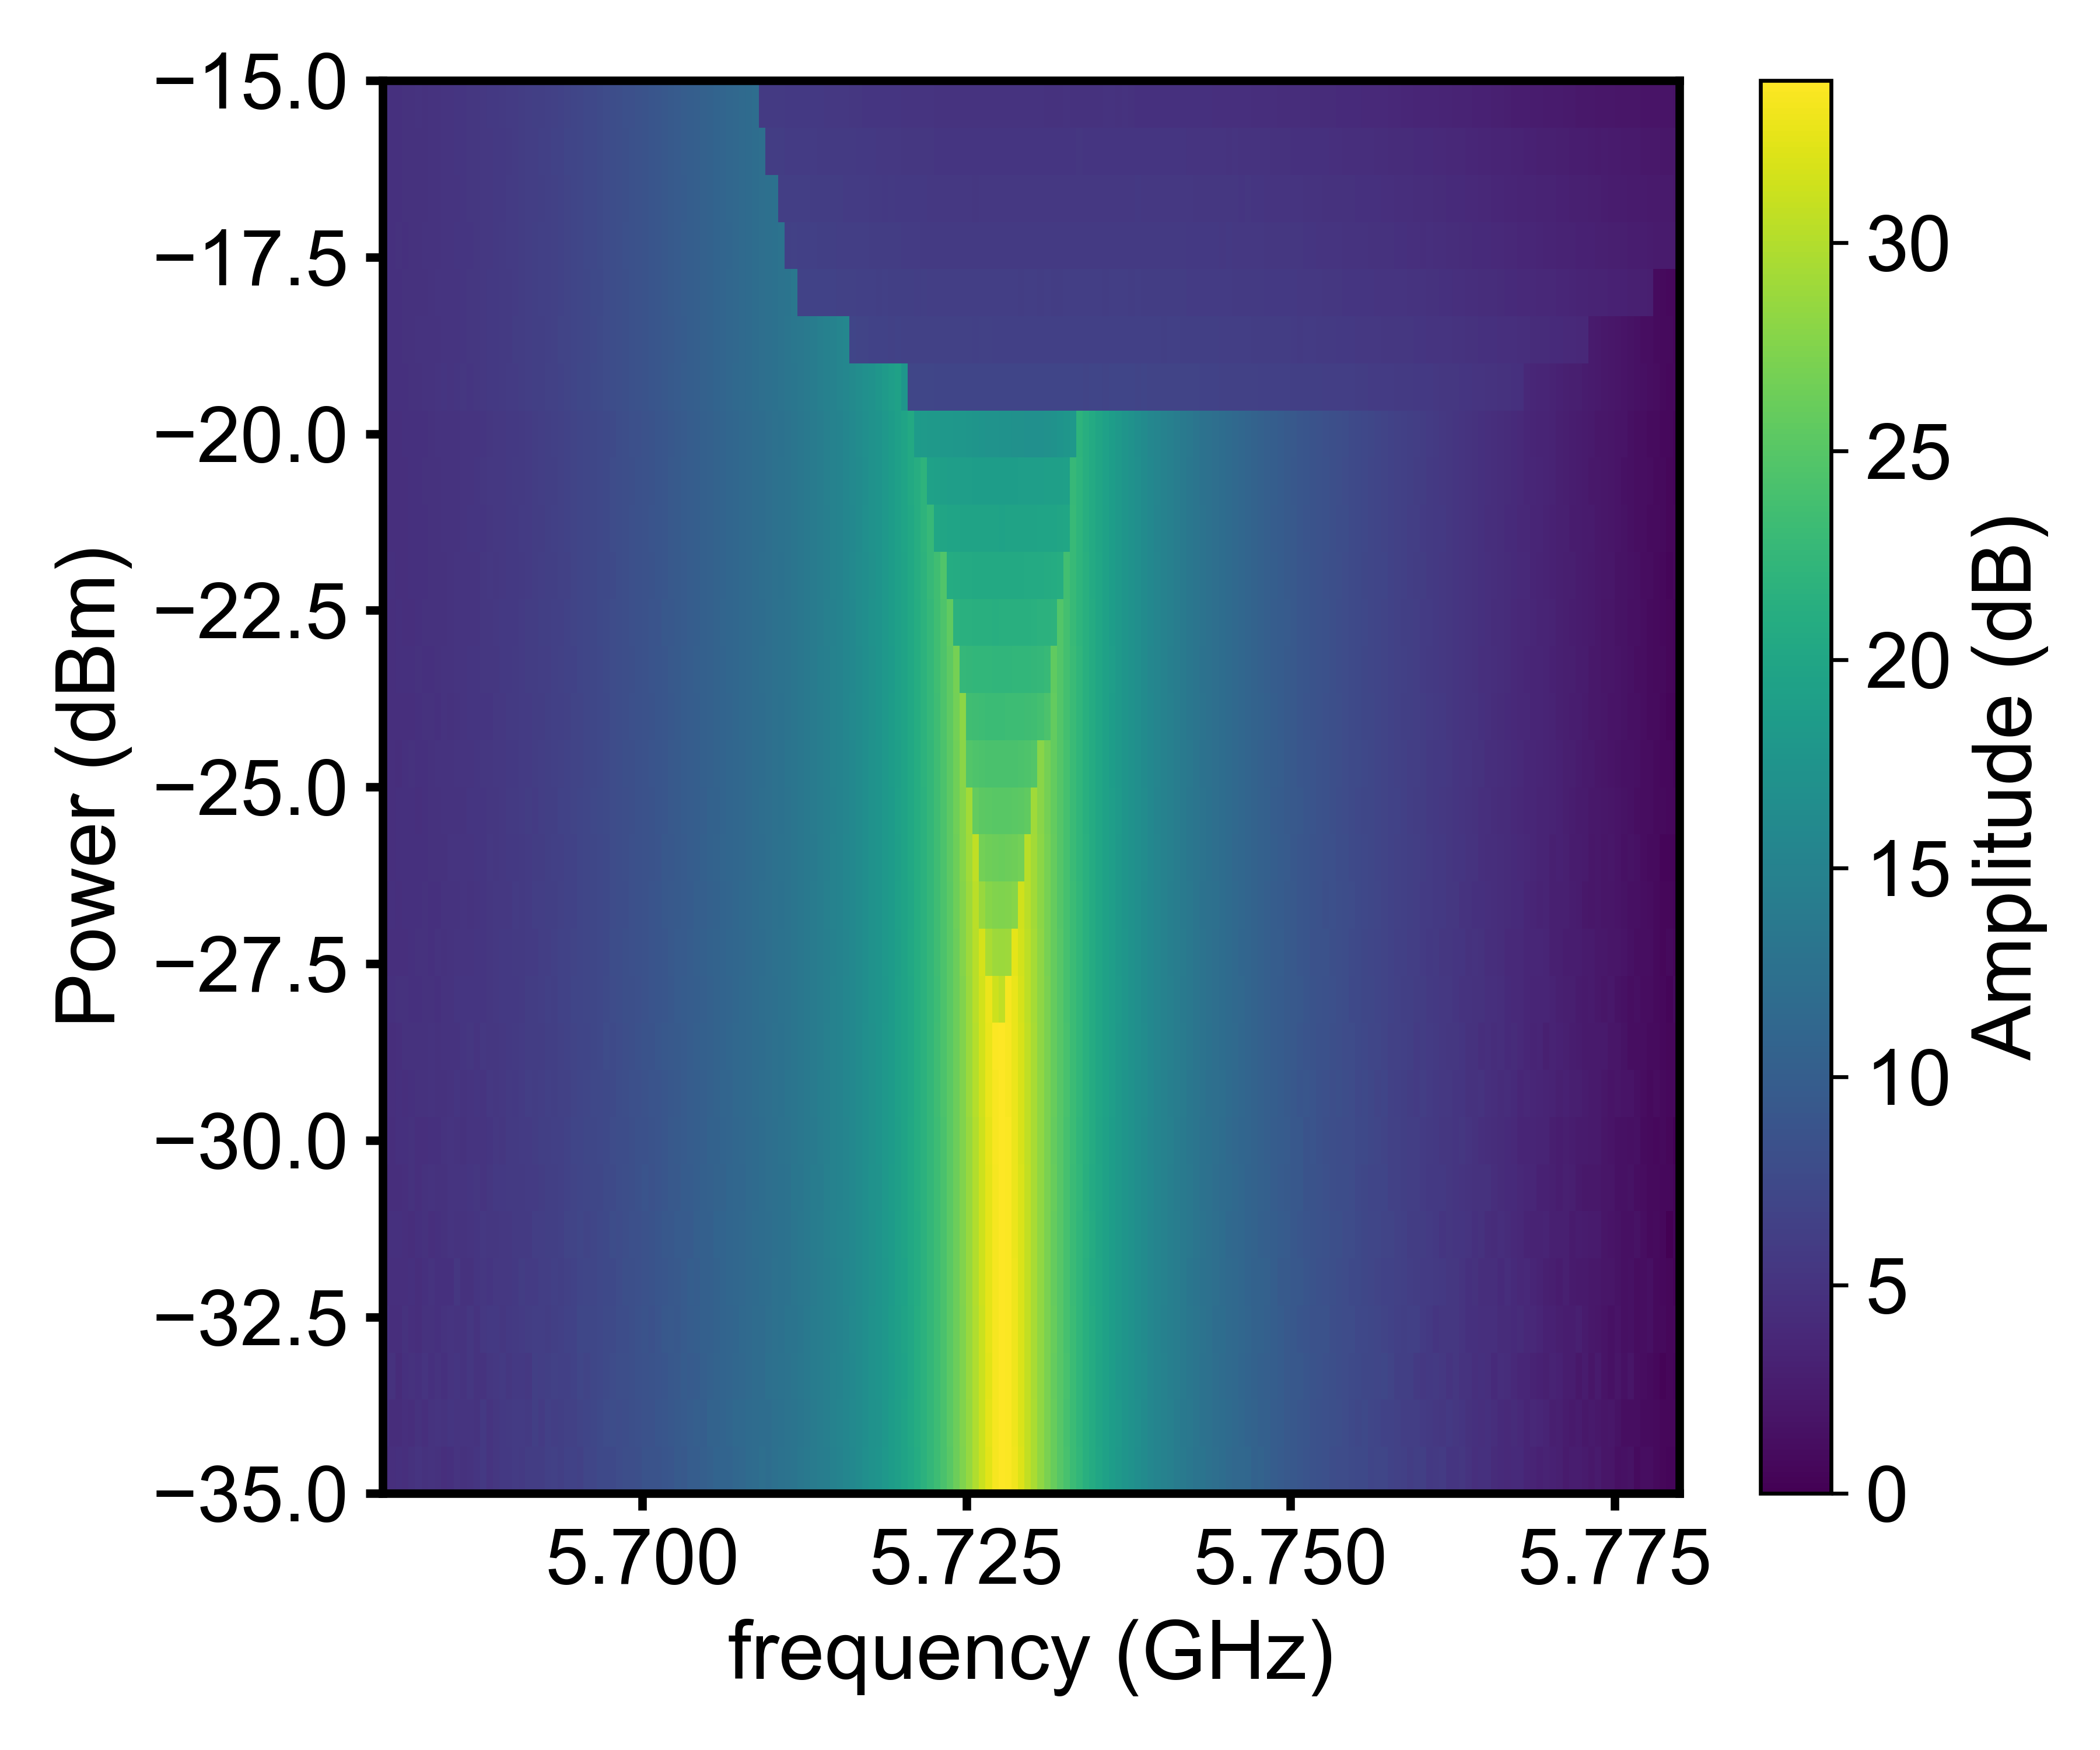
\includegraphics[width=0.6\textwidth]{polished/power_mag.png}
	\caption[Flip-flop qubit turn on and pinch-off]{\textbf{Flip-flop qubit turn on and pinch-off. a}}
	\label{fig:res_power}
\end{figure}


\subsection{Charge qubit} \label{sec:res_chargequbit}
